\documentclass[10pt]{article}
\usepackage[margin=.7in]{geometry}
\usepackage{amsthm}
\usepackage{hyperref}
\usepackage{graphicx}
\usepackage{booktabs}
\listfiles

\begin{document}
 
\begin{center}
\large
\hfill Okeefe Niemann\\
\hfill 4/16/2014\\
\hfill 1281465\\
\hfill PHYS 115 \\
\LARGE \textbf{Assignment 3}\\
\end{center}
\normalsize
\section{Question 1}
\begin{center}
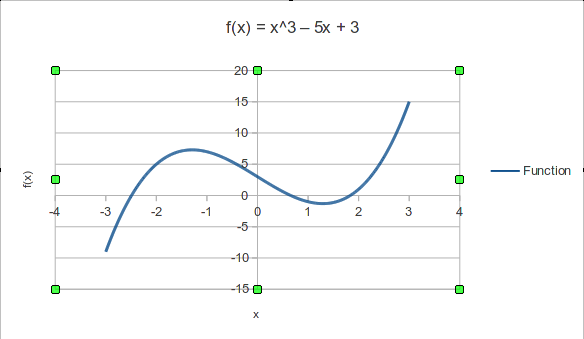
\includegraphics[scale=.7]{PHYS115week3graph}
\end{center}
\begin{itemize}
\item Input:
\begin{verbatim}
#include<stdio.h>
#include<math.h>

/* Defines Function */
double f(double x){
        return (pow(x, 4) - 5 * x + 3);
}

int main()
{
        double x_l, x_u, f(), x, y;

        x_l = .5;
        x_u = 1.5;
        printf("1st Root         f(x)\n");

/* Using bisection method, function loops until desired precision is met */
        /*Finds first positive root to e^-4 precision*/
        while (fabs(f(x)) > 1.e-4)
        {
        x = .5 * (x_l + x_u);
                if (f(x) > 0)
                        x_l = x;
                else
                        x_u = x;

        printf("%f      %.5e\n", x_l, abs(f(x_l)));
        }

        x_l = 1.5;
        x_u = 2;
        x = .5 * (x_l + x_u);
        printf("2nd Root         |f(x)|\n");
        /*Finds second positive root to e^-4 precision*/
        while (fabs(f(x)) > 1.e-4)
        {
        x = .5 * (x_l + x_u);
                if (f(x) < 0)
                        x_l = x;
                else
                        x_u = x;
        }

        printf("%f      |%.5e|\n", x_l, abs(f(x_l)));

return 0;

}
\end{verbatim}
\item Output:
\begin{verbatim}
1st Root         |f(x)|
0.656616      1.56421e-05
2nd Root         f(x)
1.750000      3.90625e-01

\end{verbatim}
\textbf{Comment:} The above output represents the two roots found to a precision, which itself is given by the deviation from zero when the function is evaluated at the root (ie f(x)).

\end{itemize}
%%%%%%%%%%%%%%%%%%%%%%%%%%%%%%%%%%%%%%%%%%%%%%%%%%%%%%%%%%%%%%%%%%%%%%%%%%%%%%%%%%%%%%
\section{Question 2}
\begin{itemize}
\item Input:
\begin{verbatim}
#include<stdio.h>
#include<math.h>

/*original function from question 1*/
double f(double x)
{
        return (pow(x, 3) - 5 * x + 3);
}

/*derivative of the function from question 1*/
double g(double x)
{
        return (3*pow(x, 2) - 5);
}

int main()
{
        double x, f(), g(), EPS;

        /*desired precision*/
        EPS = 1.e-14;
        /*value of 1st root using bisection method*/
        x = 0.656616;
        
        printf("        x               f(x)\n");
        printf("1st root:\n");

        /*loops NR method on 1st root until desired precision is achieved*/
        while (fabs(f(x)) > EPS)
        {
                x -= (f(x)/g(x));
        }
        printf(" %.14f    %e \n", x, f(x));
        
        /*value of 2nd root using bisection method*/
        x = 1.834229;
        
        printf("\n2nd root:\n");
        
        /*loops NR method on 2nd root until desired precision is achieved*/
        while (fabs(f(x)) > EPS)
        {
                x -= (f(x)/g(x));
        }
        printf(" %.14f    |%e| \n", x, f(x));

return 0;
}
\end{verbatim}
\item Output:
\begin{verbatim}
        x              |(f(x)|
1st root:
 0.65662043104711    4.440892e-16 

2nd root:
 1.83424318431392    8.881784e-16 
\end{verbatim}
\end{itemize}
\textbf{Comment:} For both roots, there was only two iterations before the desired precision was achieved, which shows the efficiency of the Newton-Raphson method.

%%%%%%%%%%%%%%%%%%%%%%%%%%%%%%%%%%%%%%%%%%%%%%%%%%%%%%%%%%%%%%%%%%%%%%%%%%%%%%%%%%%%%%%%
\section{Question 3}
\begin{itemize}
\item Input:
\begin{verbatim}
#include<stdio.h>
#include<math.h>

/*function used for this question*/
double f(double x)
{
        return (x - tanh(2*x));
}

main()
{
        double x, f(), x_n, x_m, EPS;
        
        x_n = 0.5;  /*x_(n-1)*/
        x_m = 1.5;  /*x_n*/
        EPS = 1.e-12;   /*desired precision*/
        x= 1;
        
        printf("    x          |f(x)|\n");
        
        /*Using the secant method, loops the given function for its root until 
        desired precision is achieved*/
        while (fabs(f(x)) > EPS)
        {
                x = x_m - f(x_m)*(x_m - x_n)/(f(x_m) - f(x_n));
                x_n = x_m;
                x_m = x;         
        }
        printf("%f     %.5e\n", x, fabs(f(x)));
}
\end{verbatim}
\item Output:
\begin{verbatim}
    x          |f(x)|
0.957504     2.22045e-15
\end{verbatim}
\end{itemize}

%%%%%%%%%%%%%%%%%%%%%%%%%%%%%%%%%%%%%%%%%%%%%%%%%%%%%%%%%%%%%%%%%%%%%%%%%%%%%%%%%%%%%%%%%%%
\section{Question 4}
\begin{itemize}
\item Input:
\begin{verbatim}
#include<stdio.h>
#include<math.h>

/*function whose root is the square root of 2*/
double f(double x)
{
        return (2 - pow(x,2));
}

/*derivative of the above function*/
double g(double x)
{
        return (-2*x);
}

int main()
{
        double x, f(), g(), EPS;
        
        /*desired precision*/
        EPS = 1.e-14;
        x = 1.5;
        
        printf("        x               |f(x)|\n");
        
        /*loops NR method on defined function until desired precision is achieved*/
        while (fabs(f(x)) > EPS)
        {
                x -= (f(x)/g(x));
        }
        printf(" %.14f    %e \n", x, fabs(f(x)));
return 0;
}
\end{verbatim}
\item Output:
\begin{verbatim}
      x               |f(x)|
 1.41421356237310    4.440892e-16 
\end{verbatim}
\end{itemize}

%%%%%%%%%%%%%%%%%%%%%%%%%%%%%%%%%%%%%%%%%%%%%%%%%%%%%%%%%%%%%%%%%%%%%%%%%%%%%%%%%%%%%%%%
\section{Question 5}
\begin{itemize}
\item Input:
\begin{verbatim}
#include<stdio.h>
#include<math.h>

//Establishes the value f(y) for given differential equation dy/dx
double f(double y)
{
        return (pow(y,2) + 1);
}

int main()
{
        double y2, y1, y0, h, k1, k2, f(), b, a, exact;
        int i, n;
        
        //limits of integration
        a = 0;
        b = M_PI_4;
        //condition for y=0
        y0 = 0;
        //analytical value of integral
        exact = 1;

        printf("Value of Integral         (y2-exact)/h^2        n\n");


        for (n = 1; n < 100000; n*=2)
        {
                h = (b - a) / n;
                //establishes first iteration by euler's method
                y2 = y0 + (h * f(y0));
                
                for (i = 1; i < n; i++)
                {
                        //Runge-Kutta Method 2
                        y1 = y2;	               //creates recursive relationship
                        k1 = f(y1);				   //defines k1
                        k2 = f(y1 + h * k1);	   //defines k2
                        y2 = y1 + h/2 * (k1 + k2); //evaluates higher precision value for y
                }
                printf("   %f               %.2e       %d\n", y2, fabs((y2 - exact)/pow(h, 2)), n);
                
        }

return 0;
}
\end{verbatim}
\item Output:
\begin{verbatim}
Value of Integral    (y2-exact)/h^2        n
   0.78539816          3.48e-01        1
   0.95619405          2.84e-01        2
      ...                ...           ...
   1.00000001          4.67e-02        2048
   1.00000000          4.70e-02        4096
   1.00000000          4.71e-02        8192
   1.00000000          4.71e-02        16384
   1.00000000          4.72e-02        32768
   1.00000000          4.72e-02        65536

\end{verbatim}

\end{itemize}

\textbf{Comment:} A number of iterations were omitted to save paper space, but as can be seen in the output, the error tends to a constant as the iterations go to high values. In addition, although rk2 is self starting, I was able to use the first step of the Euler method because its error is also of order $h^2$. 

%%%%%%%%%%%%%%%%%%%%%%%%%%%%%%%%%%%%%%%%%%%%%%%%%%%%%%%%%%%%%%%%%%%%%%%%%%%%%%%%%%%%%%%%%%%%%%%%%%%%%%%%%%%%%%%%%%%%%%%%%%%%%%%%%%%%%%%%

\section{Question 6}
\begin{itemize}
\item Input:

\begin{verbatim}
#include<stdio.h>
#include<math.h>

//establishes function for the derivatives of x and p
void derivs(double t, double x[], double dxdt[])
{
        dxdt[0] = x[1];           //dxdt = p
        dxdt[1] = -x[0]*x[0]*x[0];  //dpdt = -x^3
}

//establishes function for Runge-Kutta Method  2
void rk2 (double t, double x[], void derivs(double, double[], double[]), double h, int M) 
{

        double k1[M], k2[M], xp[M];
        int i;
        
        derivs(t, x, k1); 
// compute k1[i] (= derivs at (t, x) )

        for (i=0; i < M; i++) 
                xp[i] = x[i] + h * k1[i]; 
// xp = x + h*k1

        derivs(t+h, xp, k2); 

// compute k2[i] (= derivs at (t+h, x+h*k1) )
 
        for(i=0; i < M; i++) 
                x[i] += 0.5 * h * (k1[i] + k2[i]); 
// compute x[i]
}

main()
{
 
        int M = 2; 
// specify the no. of variables
 
        double t, x[M], h, tn, t0, en; 
// x is an array of size M
 
        void derivs(); 
// derivs computes the derivatives

         int n, i, j, k;

         double x_max[3] = {0.1, 1, 10};
// maximum amplitudes which will be applied to rk2

for (k = 0; k < 3; k++)
{
        x[0] = x_max[k];
        //implements maximum amplitude

        printf("\nMaximum amplitude: %.2f\n", x[0]);
        printf("  Time      Position    Momentum\n");
        
        x[1] = 0; //initializes p = 0
        t0 = 0; 
        n = 50000; //number of steps
        h = .001; //length of each step
        t = t0;

        /*loop below identifies where the first root of the oscillating
        function is located, which can then be multiplied by four to find
        the length of its period.*/

        for (i = 0; i < n; i++)
        {
                rk2(t, x, derivs, h, M); 
                // Call RK2
                if (x[0] >= 0)
                {
                        t += h;
                }
                else
                        break;
        }

        /*now that the period is found, can define tn and subsequently h*/
        
        tn = 4 * t;
        n = 50;
        t0 = 0;
        h = (tn - t0) / n;
        t = t0;
        
        for (j = 0; j < n; j++)
        {
                //Calls rk2
                rk2(t, x, derivs, h, M);
                //increments time by h until full period is reached
                t += h;
                printf("%f   %f   %f\n", t, x[0], x[1]);
        }
}

return 0;
}
\end{verbatim}
\item Output:
\begin{verbatim}
Maximum amplitude: 0.10
 Time   Position  Momentum
1.483   -0.010   -0.007
2.966   -0.021   -0.007
 ...      ...      ...
19.282   -0.100   0.001
20.765   -0.097   0.002
 ...      ...      ...
37.080   0.001   0.007
38.563   0.012   0.007
 ...      ...      ...
56.362   0.099   -0.001
57.845   0.097   -0.002
 ...      ...      ...
74.160   -0.003   -0.007

Maximum amplitude: 1.00
 Time   Position  Momentum
0.148   -0.106   -0.707
0.297   -0.210   -0.706
 ...      ...     ...
1.928   -0.995   0.085
2.076   -0.972   0.228
 ...      ...     ...
3.708   0.015   0.709
3.856   0.120   0.709
 ...     ...      ...
5.636   0.994   -0.108
5.784   0.968   -0.250
 ...     ...      ...
7.416   -0.033   -0.711

Maximum amplitude: 10.00
 Time   Position  Momentum
0.015   -1.089   -70.702
0.030   -2.135   -70.621
 ...      ...     ...  
0.192   -9.952   8.578
0.207   -9.717   22.892
 ...      ...     ...
0.370   0.131   70.893
0.385   1.180   70.881
 ...      ...     ...
0.562   9.951   -10.095
0.577   9.694   -24.356
 ...     ...      ...
0.740   -0.254   -71.076
\end{verbatim}
\end{itemize}
\textbf{Comment:}As is shown in the output, the period for maximum amplitude .1 is 74.2, maximum amplitude 1 is 7.42, and maximum amplitude 10 is 0.740. Based on these results, the period tends to be proportional to one over the maximum amplitude.


%%%%%%%%%%%%%%%%%%%%%%%%%%%%%%%%%%%%%%%%%%%%%%%%%%%%%%%%%%%%%%%%%%%%%%%%%%%%%%%%%%%%%%%
\section{Question 7}
\begin{itemize}
\item Input:
\begin{verbatim}
#include<stdio.h>
#include<math.h>

/*Establishes the value f(y) for given differential equation dy/dx*/
double f(double y)
{
        return (pow(y,2) + 1);
}

int main()
{
        double y2, y1, y0, h, k1, k2, k3, k4, f(), b, a, exact;
        int i, n;
        
        /*limits of integration*/
        a = 0;
        b = M_PI_4;
        /*condition for y=0*/
        y0 = 0;
        /*analytical value of integral*/
        exact = 1;
        
        printf("Value of Integral      (y2 - exact)/h^4      n\n");
        
        for (n = 1; n <= 140; n++)  /*increases the number of bins each iteration*/
        {
                h = (b - a) / n;
                y2 = y0;
                
                for (i = 1; i <= n; i++)
                {
                        /*Runge-Kutta Method 4*/
                        y1 = y2;	                    /*creates recursive relationship*/
                        k1 = f(y1);				        /*defines k1*/
                        k2 = f(y1 + h / 2 * k1);	    /*defines k2*/
                        k3 = f(y1 + h / 2 * k2);		/*defines k3*/
                        k4 = f(y1 + h * k3);			/*defines k4*/
                        y2 = y1 + h / 6 * (k1 + 2*k2 + 2*k3 + k4); 
                }
                printf("   %f               %.2e           %d\n", y2, fabs((y2 - exact)/pow(h, 4)), n);
                
        }

return 0;
}
\end{verbatim}
\item Output:
\begin{verbatim}
Value of Integral      (y2 - exact)/h^4      n
   0.996887               8.18e-03           1
   0.999836               6.89e-03           2
   0.999983               3.55e-03           3
   0.999999               9.03e-04           4
   1.000001               1.09e-03           5
   1.000001               2.60e-03           6
     ...                    ...              ...
   1.000000               1.22e-02           135
   1.000000               1.22e-02           136
   1.000000               1.22e-02           137
   1.000000               1.22e-02           138
   1.000000               1.22e-02           139
   1.000000               1.22e-02           140
\end{verbatim}

\textbf{Comment:}As can be seen in the above output, the error of RK4 divided by $h^4$ tends to a constant. 
\end{itemize}


\end{document}
